\documentclass[
  bibliography=totoc,     % Literatur im Inhaltsverzeichnis
  captions=tableheading,  % Tabellenüberschriften
  titlepage=firstiscover, % Titelseite ist Deckblatt
]{scrartcl}

% Vektoren
\usepackage{esvect}


% Paket float verbessern
\usepackage{scrhack}

% Warnung, falls nochmal kompiliert werden muss
\usepackage[aux]{rerunfilecheck}

% unverzichtbare Mathe-Befehle
\usepackage{amsmath}
% viele Mathe-Symbole
\usepackage{amssymb}
% Erweiterungen für amsmath
\usepackage{mathtools}

% Fonteinstellungen
\usepackage{fontspec}
% Latin Modern Fonts werden automatisch geladen
% Alternativ zum Beispiel:
%\setromanfont{Libertinus Serif}
%\setsansfont{Libertinus Sans}
%\setmonofont{Libertinus Mono}

% Wenn man andere Schriftarten gesetzt hat,
% sollte man das Seiten-Layout neu berechnen lassen
\recalctypearea{}

% deutsche Spracheinstellungen
\usepackage{polyglossia}
\setmainlanguage{german}

% Blindtext
\usepackage{blindtext}
\usepackage{lipsum}

\usepackage[
  math-style=ISO,    % ┐
  bold-style=ISO,    % │
  sans-style=italic, % │ ISO-Standard folgen
  nabla=upright,     % │
  partial=upright,   % ┘
  warnings-off={           % ┐
    mathtools-colon,       % │ unnötige Warnungen ausschalten
    mathtools-overbracket, % │
  },                       % ┘
]{unicode-math}

% traditionelle Fonts für Mathematik
\setmathfont{Latin Modern Math}
% Alternativ zum Beispiel:
%\setmathfont{Libertinus Math}

\setmathfont{XITS Math}[range={scr, bfscr}]
\setmathfont{XITS Math}[range={cal, bfcal}, StylisticSet=1]

% Zahlen und Einheiten
\usepackage[
  locale=DE,                   % deutsche Einstellungen
  separate-uncertainty=true,   % immer Fehler mit \pm
  per-mode=symbol-or-fraction, % / in inline math, fraction in display math
]{siunitx}

% chemische Formeln
\usepackage[
  version=4,
  math-greek=default, % ┐ mit unicode-math zusammenarbeiten
  text-greek=default, % ┘
]{mhchem}

% richtige Anführungszeichen
\usepackage[autostyle]{csquotes}

% schöne Brüche im Text
\usepackage{xfrac}
\usepackage{nicefrac}

% Standardplatzierung für Floats einstellen
\usepackage{float}
\floatplacement{figure}{htbp}
\floatplacement{table}{htbp}

% Floats innerhalb einer Section halten
\usepackage[
  section, % Floats innerhalb der Section halten
  below,   % unterhalb der Section aber auf der selben Seite ist ok
]{placeins}

% Seite drehen für breite Tabellen: landscape Umgebung
\usepackage{pdflscape}

% Captions schöner machen.
\usepackage[
  labelfont=bf,        % Tabelle x: Abbildung y: ist jetzt fett
  font=small,          % Schrift etwas kleiner als Dokument
  width=0.9\textwidth, % maximale Breite einer Caption schmaler
]{caption}
% subfigure, subtable, subref
\usepackage{subcaption}

% Grafiken können eingebunden werden
\usepackage{graphicx}
% größere Variation von Dateinamen möglich
\usepackage{grffile}

% schöne Tabellen
\usepackage{booktabs}

% Verbesserungen am Schriftbild
\usepackage{microtype}

% Literaturverzeichnis
\usepackage[
  backend=biber,
]{biblatex}
% Quellendatenbank
\addbibresource{lit.bib}
\addbibresource{programme.bib}

% Hyperlinks im Dokument
\usepackage[
  unicode,        % Unicode in PDF-Attributen erlauben
  pdfusetitle,    % Titel, Autoren und Datum als PDF-Attribute
  pdfcreator={},  % ┐ PDF-Attribute säubern
  pdfproducer={}, % ┘
]{hyperref}
% erweiterte Bookmarks im PDF
\usepackage{bookmark}

% Trennung von Wörtern mit Strichen
\usepackage[shortcuts]{extdash}
%Erlaubt Einfügen von PDF-Dateien
\usepackage{pdfpages}

% Micro in \SI{}{} reparieren
\sisetup{math-micro=\text{µ},text-micro=µ}

\author{%
  Lars Kolk\\%
  \href{mailto:lars.kolk@tu-dortmund.de}{lars.kolk@tu-dortmund.de}%
  \texorpdfstring{\and}{,}%
  Julia Sobolewski\\%
  \href{mailto:julia.sobolewski@tu-dortmund.de}{julia.sobolewski@tu-dortmund.de}%
}
\publishers{TU Dortmund – Fakultät Physik}

\usepackage{longtable}
\usepackage{wrapfig}
\usepackage{ dsfont }
\subject{VERSUCH 401}
\title{Das Michelson-Interferometer}
\date{%
  \hspace{-2.5em}
  Durchführung: 26.06.2018
  \hspace{4em}
  Abgabe: 03.07.2018
}

\begin{document}
  \setlength{\parindent}{0em}
  \maketitle
  \thispagestyle{empty}
  \newpage
  \tableofcontents
  \newpage


\section{Ziel}
In diesem Versuch soll die Ablenkung eines Elektronenstrahls im elektrischen und magnetischen Feld untersucht werden.
\section{Theorie}
\subsection{Aufbau einer Kathodenstrahlröhre}
Die Kathodenstrahlröhre besteht aus drei Teilen: der sogenannten Elektronenkanone, einem Ablenk- und einem Nachweissystem.
Die Elektronenkanone erzeugt freie Elektronen durch Glühemission.
Die dabei erhitzte Kathode wird von einem Wehnelt-Zylinder umgeben, der in Abbildung \ref{fig:WZ} dargestellt wird.
\begin{figure}[H]
  \centering
  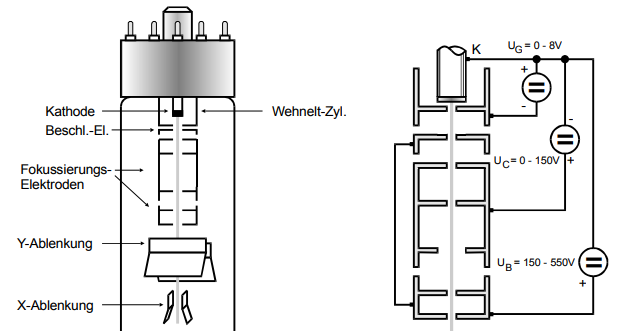
\includegraphics[width=\linewidth-100pt,height=\textheight-100pt,keepaspectratio]{Text/Bilder/Kathodenstrahlroehre.png}
  \caption{Querschnitt durch eine Kathodenstrahlröhre und die Beschaltung ihrer „Elektronenkanone" \cite[82]{sample}}
  \label{fig:WZ}
\end{figure}
Aufgrund der Potentialdifferenz zwischen Kathode und dem Wehnelt-Zylinder, steuert letzterer die Intensität des Elektronenstrahls.
Zusätzlich befindet sich vor diesem eine Elektrode mit hohen positiven Potential gegenüber der Kathode. Diese beschleunigt die Elektronen auf die Geschwindigkeit
\begin{equation}
  v=\sqrt{\frac{2 e_0 U_B}{m}} \text{.} \label{eqn:vnk}
\end{equation}
Nachdem die Elektronen auf diese Geschwindigkeit beschleunigt wurden, werden sie durch sich an den Seiten befindenden Elektroden, den Elektronenlinsen, abgelenkt und fokussiert.
Bevor die Elektronen jedoch den Leuchtschirm erreichen, passieren sie das Ablenksystem. Dieses besteht aus zwei je paralellen Plattenpaaren, in denen der Elektronenstrahl durch elektrische Felder in X- bzw Y-Richtung
abgelenkt wird. Dies wird in \ref{sec:AiE} näher erläutert.
Danach treffen die Elektronen auf den Leuchtschirm, auf dem ihre Position durch emittierte Lichtquanten sichtbar gemacht wird. Zur Emission kommt es durch Anregung der Aktivatorzentren im Schirm, d.h. Störstellen im Gitter
des Materials. Damit der Schirm elektrisch neutral bleibt, ist dieser mit der Beschleunigungselektrode verbunden.
\subsection{Ablenkung im E-Feld} \label{sec:AiE}
Bei einem Plattenpaar mit Abstand $d$ und Länge $l$ kann für den Fall $d \ll l$ das Feld zwischen den Platten mit
\begin{equation}
E=\frac{U_d}{d}
\end{equation}
als konstant genähert werden. Das Elektron erfährt dann die Kraft
\begin{equation}
  F= \left | \vec{E}\cdot e_0 \right | = e_0 \cdot \frac{U_d}{d}
\end{equation}
über einen Zeitraum $\Delta t$. Damit wird es, wie in Abbildung \ref{fig:SidK} zu sehen ist, konstant in y-Richtung abgelenkt.
Da $F$ konstant ist, gilt mit $v=a_y \cdot \Delta t$ und $a_y = F/m_0$ :
\begin{equation}
  v_y=\frac{e_0}{m_0}\frac{U_d}{d}\Delta t \label{eqn:bla}
\end{equation}
Aus Abbildung \ref{fig:SidK} lassen sich zusätzlich die Zusammenhänge $\Delta t =\frac{p}{v_z}$ und $\theta=\frac{v_y}{v_z}$
entnehmen, womit \eqref{eqn:bla} umgeschrieben werden kann zu
\begin{equation}
  v_y=\frac{e_0}{m_0} \frac{U_d}{d} \frac{p}{v_z} \text{.}
\end{equation}
Damit gilt die Verschiebung
\begin{equation}
  D=\frac{e_0}{m_0} \frac{U_d}{d} \frac{p}{(v_z)^2}L =\frac{p}{2d}\frac{U_d}{U_B}L \text{.}
\end{equation}
\begin{figure}
  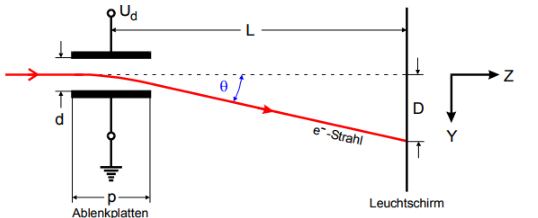
\includegraphics[width=\linewidth-100pt,height=\textheight-100pt,keepaspectratio]{Text/Bilder/Ablenkplatten.png}
  \caption{Strahlablenkung in der Kathodenstrahlröhre\cite[83]{sample}.}
  \label{fig:SidK}
\end{figure}
%Aus diesem Zusammenhang ergibt sich auch, dass für eine hohe Ablenkempfindlichkeit $L$
%und $p$ groß sein müssen, währenddessen $U_B$ klein sein muss. In diesem Fall könnten jedoch
%nur niederfequente Spannungen untersucht werden, da die Flugzeit $\Delta t$ klein gegen die
%Periodendauer von $U$ sein muss.
%Bei hochfrequenten Wechselspannungen muss dagegen $p$ klein und $U_b$ groß sein.

\subsection{Kathodenstrahl-Oszillographen}
Wird an den Platten, die den Elektronenstrahl in X-Richtung ablenken, eine Wechsel-
spannung und an das andere Plattenpaar die zu untersuchende Spannung angebracht,
so kann eine Kathodenstrahlröhre zu einem Kathodenstrahl-Oszillographen erweitert
werden. Diese erlaubt es, die Zeitabhängigkeit von Wechselspannungen darzustellen. Sind
die beiden Spannungen im passenden Verhältnis zueinander, so zeichnet sich der zeitliche
Verlauf am Laufschirm ab. Es soll gelten:
\begin{align}
  n \cdot v_\text{Sä} = m \cdot v_\text{Sig} && \text{n, m} \in \mathds{N}
\end{align}

\subsection{ Ablenkung im B-Feld}
Bewegt sich eine Ladung $q$ mit einer Geschwindigkeit $v$ verschieden von $0$ in einem magnetischen statt einem elektrischen Feld , so wirkt auf
dieses die Lorentzkraft:
\begin{equation}
  \vec{F}=q \cdot \vec{v} \times \vec{B}
\end{equation}
Im Fall $\vec{v} \bot \vec{B}$  gilt für ein Elektron:
\begin{equation}
  F_L= e_0 \cdot v \cdot B
\end{equation}

Wie in Abbildung \ref{fig:WDM} zu sehen ist, bewegen sich die Elektronen mit der in \eqref{eqn:vnk} gegebenen
Geschwindigkeit geradlinig, bis sie bis sie durch die Lorentzkraft auf eine Kreisbahn
geraten, womit diese der Zentripetalkraft $F = \frac{mv^2}{r}$
entspricht. Damit gilt für den Radius:
\begin{equation}
  r=\frac{m_0 v_0}{e_0 B}
\end{equation}
\begin{figure}[H]
  \centering
  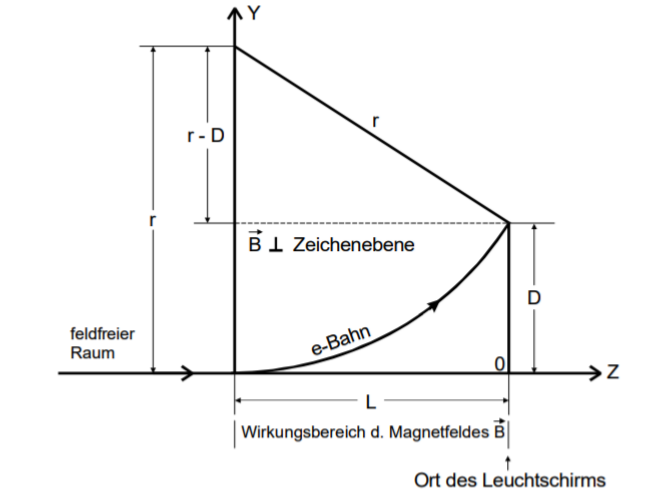
\includegraphics{Text/Bilder/WDM.png}
  \caption{ Skizze zur Ableitung einer Beziehung zwischen L, D und r \cite[89]{sample2}.}
  \label{fig:WDM}
\end{figure}
Für die in \ref{fig:WDM} zu sehende Konstallation folgt dann aus geometrischen Überlegung und \eqref{eqn:vnk} der
Zusammenhang
\begin{equation}
  \frac{D}{D^2+L^2}=\frac{1}{8U_B}\sqrt{\frac{e_0}{m_o}}B \text{.}
\end{equation}

\section{Durchführung}

\subsection{Magnetfeld von Spulen \label{sec:mvs}}
Zunächst wird die lange Spule an das Netzgerät angeschlossen. Daraufhin werden
Strom und Spannung hochgeregelt, wobei die maximale Spannung nicht überschritten werden darf.
Mithilfe einer Longitudinalsonde wird nun die magnetische Flussdichte innerhalb und außerhalb der Spule gemessen.
Dazu soll die Sonde so justiert werden, dass das Magnetfeld auf der Achse der Spule gemessen wird.
Der Messvorgang wird für die kleine Spule wiederholt.
Der experimentelle Aufbau ist in Abbildung \ref{A1} dargestellt.
\begin{figure}
  \centering
  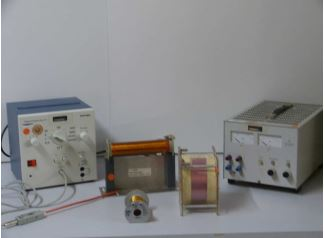
\includegraphics{Text/Bilder/Aufbau1.jpg}
  \caption{Experimenteller Aufbau \cite[4]{sample}.}
  \label{A1}
\end{figure}

\subsection{Magnetfeld von Spulenpaaren}
Ähnlich wie in Kapitel \ref{sec:mvs} wird in diesem Versuchsteil eine Helmholtz-Spule an das Netzgerät angeschlossen.
Dabei sollen beide Spulen in Reihe geschaltet werden.Die Spannung muss so gewählt werden, dass der maximal zulässige Spulenstrom
nicht überschritten wird.
Mithilfe einer transversalen Hallsonde wird die magnetische Flussdichte $\vec{B}$
für drei Spulenabstände sowohl zwischen als auch außerhalb
der Spulen gemessen.
Der experimentelle Aufbau ist in Abbildung \ref{A2} dargestellt.
\begin{figure}
  \centering
  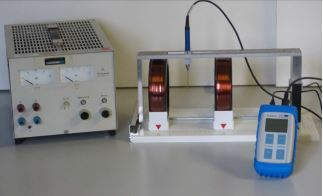
\includegraphics{Text/Bilder/Aufbau2.jpg}
  \caption{Experimenteller Aufbau \cite[5]{sample}.}
  \label{A2}
\end{figure}

\subsection{Hysteresekurve}
In diesem Versuchsteil wird das Netzgerät an eine Ringspule angeschlossen.
Erneut wird die magnetische Flussdichte $\vec{B}$ mit einer transversalen Hallsonde bestimmt.
Dazu wird hier jedoch die anliegene Spannung in regelmäßigen Abständen variiert und die Magnetische Flussdichte $\vec{B}$
mit der zugehörigen Spannung $U$ notiert.
Es werden 10-20 Messpaare aufgenommen.
Der experimentelle Aufbau ist in Abbildung \ref{A3} dargestellt.
\begin{figure}
  \centering
  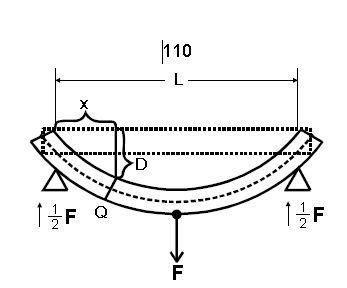
\includegraphics{Text/Bilder/Aufbau3.jpg}
  \caption{Experimenteller Aufbau \cite[5]{sample}.}
  \label{A3}
\end{figure}

\section{Auswertung}

\subsection{Bestimmung der Schallgeschwindigkeit in Acryl \label{sec:schall}}

\subsubsection{Impuls-Echo-Verfahren}

In Tabelle \ref{tab:echo} befinden sich die aufgenommenen Messwerte
\begin{table}[H]
   \centering
   \caption{Mithilfe des Impuls-Echo-Verfahrens aufgenommenen Messwerte}
   \label{tab:echo}
   \begin{tabular} { S S S S }
 \toprule
 & {Puls $1$} & {Puls $2$} \\
\cmidrule(lr){2-2} \cmidrule(lr){3-3}
 {$L\:/\: \mathrm{cm}$} & {$U\:/\: \mathrm{V}$} & {$U\:/\: \mathrm{V}$} & {$\symup{\Delta}t\:/\: \mathrm{μs}$} \\
    \midrule
    12,0 & 1,405 & 0,663 & 88,7 \\
    10,2 & 1,405 & 0,646 & 76,4 \\
    8,0 & 1,401 & 1,268 & 59,5 \\
    7,1 & 1,401 & 1,318 & 46,5 \\
    6,2 & 1,417 & 1,396 & 46,3 \\
    4,0 & 1,401 & 1,446 & 29,4 \\
    3,1 & 1,392 & 1,355 & 23,6 \\
    \bottomrule
  \end{tabular}
\end{table}


In Graph \ref{fig:echo} sind diese aufgetragen.
\begin{figure}[H]
  \centering
  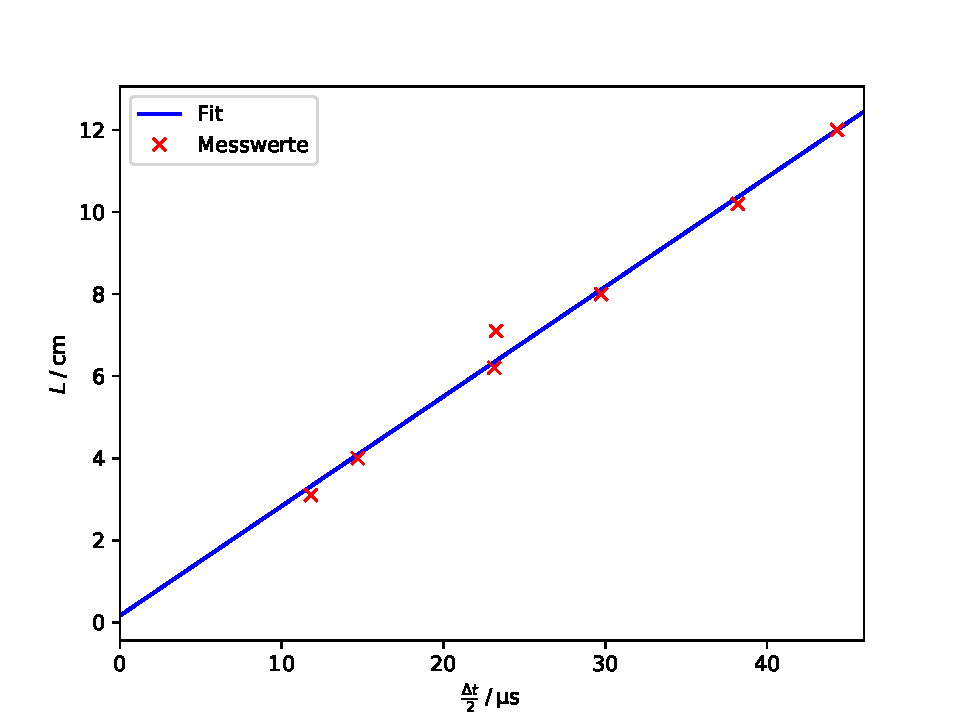
\includegraphics[width=\textwidth]{Plots/echo.pdf}
  \caption{Es ist die Länge des Acrylzylinders $L$ gegen die Zeit $\sfrac{\symup{\Delta}t}{2}$, die der Schall benötigt um diesen beim Impuls-Echo-Verfahren einmal zu durchqueren, aufgetragen.}
  \label{fig:echo}
\end{figure}

Eine lineare Regression $f(x) = a \cdot x + b$ liefert die Werte
\begin{align*}
  a &= \SI{2669,59(12355)}{\m \per \s} = c_\text{Echo} \\
  b &= \SI{0,17(35)}{\cm}.
\end{align*}

Dabei ist die Steigung $a$ die Geschwindigkeit, mit der sich der Schall durch Acryl bewegt und der y-Achsenabschnitt $b$ ist
die Dicke der Anpassungsschicht.
Der Theoriewert \cite{sample2} ist $c_\text{Acryl, theo} = \SI{2730}{\m \per \s}$, die Abweichung beträgt $\SI{2,21}{\%}$.

\subsubsection{Durchschallungs-Verfahren}

In Tabelle \ref{tab:durch} befinden sich die aufgenommenen Messwerte
\begin{table}[H]
   \centering
   \caption{Mithilfe des Durchschallungs-Verfahrens aufgenommenen Messwerte}
   \label{tab:durch}
   \begin{tabular} { S S }
 \toprule
 {$L\:/\: \mathrm{cm}$} & {$\symup{\Delta}t\:/\: \mathrm{μs}$} \\
    \midrule
    12,0 & 45,7 \\
    10,2 & 39,2 \\
    8,0 & 31,4 \\
    7,1 & 27,7 \\
    6,2 & 23,8 \\
    4,0 & 15,7 \\
    3,1 & 12,4 \\
    \bottomrule
  \end{tabular}
\end{table}


Aufgetragen sind diese in Graph \ref{fig:durch}.
\begin{figure}[H]
  \centering
  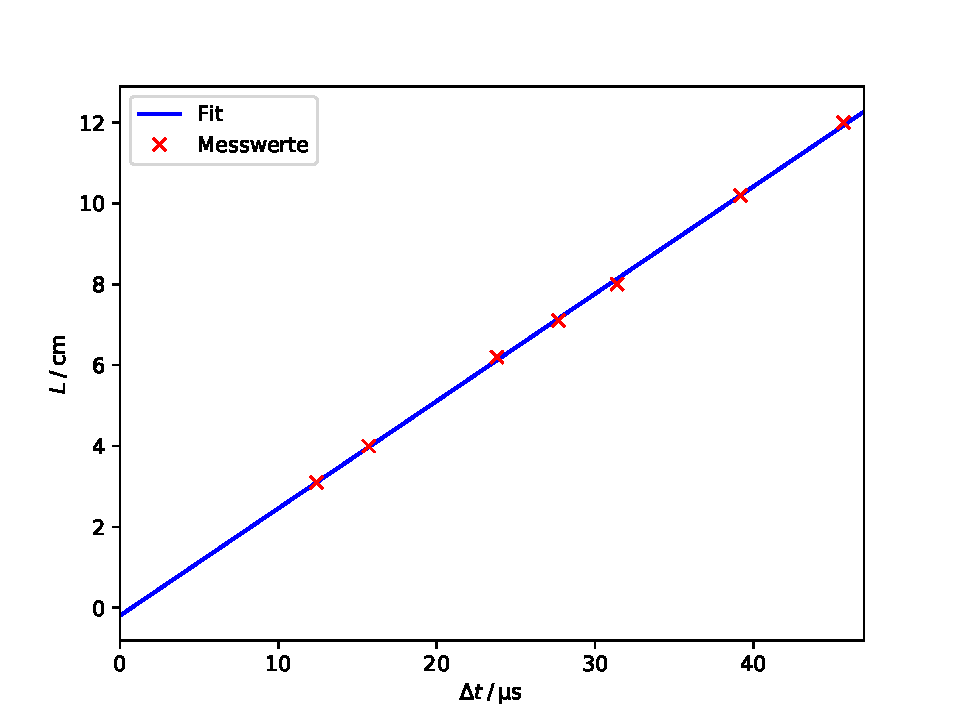
\includegraphics[width=\textwidth]{Plots/durch.pdf}
  \caption{Es ist die Länge des Acrylzylinders $L$ gegen die Zeit $\symup{\Delta}t$, die der Schall benötigt um diesen beim Durchschallungs-Verfahren einmal zu durchqueren, aufgetragen.}
  \label{fig:durch}
\end{figure}

Eine lineare Regression $f(x) = a \cdot x + b$ liefert die Werte
\begin{align*}
  a &= \SI{2652,62(2796)}{\m \per \s} = c_\text{Durch} \\
  b &= \SI{-0,19(8)}{\cm}.
\end{align*}

Dabei ist die Steigung $a$ wieder die Geschwindigkeit, mit der sich der Schall durch Acryl bewegt und der y-Achsenabschnitt $b$ ist
die Dicke der Anpassungsschicht. Die Abweichung zum Theoriewert \cite{sample2} beträgt $\SI{2,83}{\%}$.

Der Mittelwert beträgt
\begin{equation*}
  \bar{c}_\text{Acryl} = \frac{c_\text{Echo}+c_\text{Durch}}{2} = \SI{2661,10(6334)}{\m \per \s}.
\end{equation*}

Der Fehler ergibt sich aus der Gauß'schen Fehlerfortpflanzung
\begin{equation*}
  \sigma_{\bar{c}_\text{Acryl}} = \sqrt{\left( \frac{1}{2} \sigma_{c_\text{Echo}} \right)^2 + \left( \frac{1}{2} \sigma_{c_\text{Durch}} \right)^2}
\end{equation*}

Der Mittelwert weicht um $\SI{2,52}{\%}$ vom Theoriewert \cite{sample2} ab.

\subsection{Bestimmung des Dämpfungskoeffizienten mithilfe des Impuls-Echo-Verfahrens \label{sec:daem}}

In Abbildung \ref{fig:däm} sind die Werte aus Tabelle \ref{tab:echo} aufgetragen.
\begin{figure}[H]
  \centering
  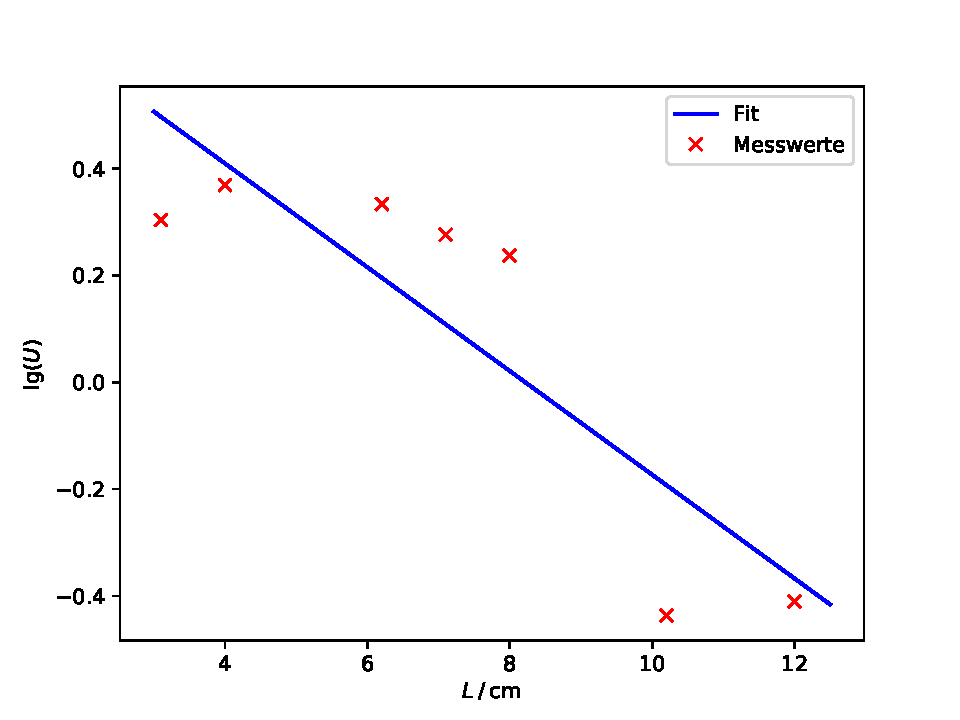
\includegraphics[width=\textwidth]{Plots/daem.pdf}
  \caption{$\ln{(U)}$-$L$-Diagramm zur Bestimmung des Dämpfungskoeffizienten}
  \label{fig:däm}
\end{figure}

Eine lineare Regression $f(x) = -a \cdot x + b$ liefert folgende Werte
\begin{align*}
  a &= \SI{-9,71(28)}{\per \m} = - \alpha \\
  b &= \SI{0,8(2)}{}.
\end{align*}

Der Dämpfungsfaktor in Acryl ist somit $\alpha = \SI{9,71(28)}{\per \m}$. Der Theoriewert \cite{sample4} beträgt $\alpha_\text{theo} = \SI{57}{\per \m}$,
wodurch sich eine Abweichung von $\SI{82,96}{\%}$ ergibt.

\subsection{Bestimmung der Dicke zweier Acrylplatten mithilfe des Cepstrums und des A-Scans \label{sec:cep}}

Die aufgenommenen Messwerte befinden sich in Tabelle \ref{tab:cep}.
\begin{table}[H]
   \centering
   \caption{Aus dem Cepstrum und A-Scan bestimmte Laufzeiten durch zwei Acrylplatten}
   \label{tab:cep}
   \begin{tabular} { c S S }
 \toprule
  & {$\symup{\Delta}t_\text{Cep} \:/\: \mathrm{μs}$} & {$\symup{\Delta}t_\text{Scan}\:/\: \mathrm{μs}$} \\
    \midrule
    $\symup{\Delta}t_1$ & 4,90 & 4,8 \\
    $\symup{\Delta}t_2$ & 8,74 & 8,6 \\
    $\symup{\Delta}t_3$ & 13,21 & 13,4 \\
    \bottomrule
  \end{tabular}
\end{table}


In Abbildung \ref{fig:cep} sind Das FTT und das Cepstrum zu sehen.
\begin{figure}[H]
  \centering
  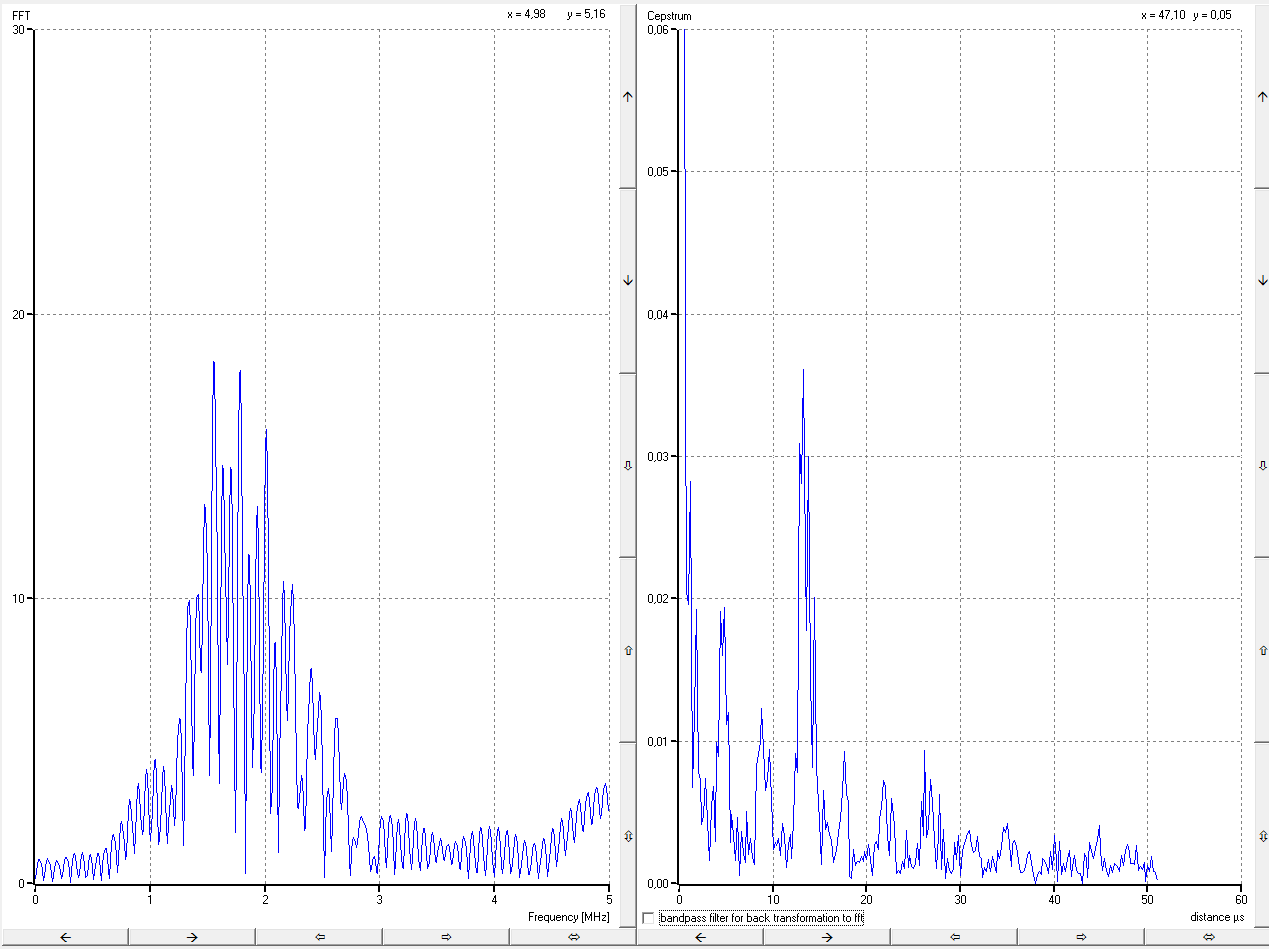
\includegraphics[width=\textwidth]{Text/Bilder/FTT,Cep.png}
  \caption{Screenshot des aufgenommenen FTT und Cepstrum}
  \label{fig:cep}
\end{figure}

Aus den gemessenen Laufzeiten werden nun die Dicken der einzelnen Platten und deren Gesamtdicke nach Gleichung \eqref{eqn:dicke} berechnet.
\begin{equation}
  d = \frac{\symup{\Delta}t}{2} \bar{c}_\text{Acryl}
  \label{eqn:dicke}
\end{equation}

Für die aufgenommenen Zeiten ergibt sich:
\begin{align*}
  d_{1, \text{Cep}} &= \SI{0,652(16)}{\cm} & d_{1, \text{Scan}} &= \SI{0,639(15)}{\cm} \\
  d_{2, \text{Cep}} &= \SI{1,163(28)}{\cm} & d_{2, \text{Scan}} &= \SI{1,144(27)}{\cm} \\
  d_{3, \text{Cep}} &= \SI{1,76(4)}{\cm} & d_{3, \text{Scan}} &= \SI{1,78(4)}{\cm}
\end{align*}

Die Mittelwerte und ihre Fehler ergeben sich aus den Gleichungen \eqref{eqn:dmit} und \eqref{eqn:derr}.
\begin{align}
  \bar{d} &= \frac{d_\text{Cep} + d_\text{Scan}}{2} \label{eqn:dmit} \\
  \sigma_{\bar{d}} &= \sqrt{\frac{1}{1 \cdot 2}  \left((\bar{d}-d_\text{Cep})^2+(\bar{d}-d_\text{Scan})^2 \right)} \label{eqn:derr}
\end{align}

Die Mittelwerte sind somit
\begin{align*}
  \bar{d}_1 &= \SI{0,645(15)}{\cm} \\
  \bar{d}_2 &= \SI{1,154(27)}{\cm} \\
  \bar{d}_3 &= \SI{1,77(4)}{\cm}.
\end{align*}

Die Abweichungen von den mithilfe der Schiebelehre bestimmten Werte
\begin{align*}
  d_{1, \text{theo}} &= \SI{0,6}{\cm} \\
  d_{2, \text{theo}} &= \SI{1,2}{\cm} \\
  d_{3, \text{theo}} &= \SI{1,8}{\cm}
\end{align*}

liegen bei $\SI{7,55}{\%}$ für $ d_1$, $\SI{3,87}{\%}$ für $d_2$ und $\SI{1,65}{\%}$ für $d_3$.

\subsection{Biometrische Untersuchung eines Augenmodells}

Die aufgenommenen Messwerte befinden sind
\begin{align*}
  \symup{\Delta}t_1 = 12,\!1 \: \symup{\mu s} \\
  \symup{\Delta}t_2 = 17,\!8 \: \symup{\mu s} \\
  \symup{\Delta}t_3 = 26,\!9 \: \symup{\mu s} \\
  \symup{\Delta}t_4 = 70,\!5 \: \symup{\mu s} \\
\end{align*}

Die jeweiligen Schallgeschwindigkeiten betragen
\begin{align*}
  c_\text{K} &= \SI{1483}{\m \per \s} \\
  c_\text{L} &= \SI{2500}{\m \per \s} \\
  c_\text{GK} &= \SI{1410}{\m \per \s}.
\end{align*}

Dabei ist $c_\text{L}$ die Schallgeschwindigkeit in der Linse \cite[6]{sample}, $c_\text{GK}$ die Schallgeschwindigkeit im Glaskörper \cite[6]{sample}
und $c_\text{K}$ die Schallgeschwindigkeit in der vorderen und hinteren Augenkammer, die mit der Schallgeschwindigkeit für Wasser \cite{sample3}
angenähert wird.

Die berechneten Werte sind:
\begin{align*}
  &\text{Hornhaut - Iris:} &d_1 &= \frac{\symup{\Delta}t_1}{2} c_\text{K} = \SI{0,90}{\cm} \\
  &\text{Iris - Linsenanfang:} &d_2 &= \frac{\symup{\Delta}t_2}{2} c_\text{K} = \SI{0,42}{\cm} \\
  &\text{Linsenanfang - Linsenende:} &d_3 &= \frac{\symup{\Delta}t_3}{2} c_\text{L} = \SI{1,14}{\cm} \\
  &\text{Linsenende - Retina:} &d_4 &= \frac{\symup{\Delta}t_4}{2} c_\text{GK} = \SI{3,07}{\cm}.
\end{align*}

\section{Diskussion}
Die Methoden, bei der die Gravitation (s.\ref{sec:grav}) und Präzession (s. \ref{sec:prae}) ausgenutzt werden,
waren mit einer prozentualen Abweichung von $3,19\%$ und $3,69\%$ etwas genauer, als die Methode,
die sich die Schwingungsdauer zu Nutze macht (s. \ref{sec:schw}). Da erhält man eine Abweichung von 6,54\%.
Bei der Betrachtung der Ergebnisse müssen aber auch die potentiellen Fehlerquellen beachtet werden.
Dazu gehören:

\begin{itemize}
  \item Bei \ref{sec:grav} war die Aluminiumstange leicht verbogen,
        wodurch die Gleichgewichtslage schwer zu erkennen war.
  \item Weitere Ungenauigkeiten bei \ref{sec:grav} können ungenaue Waagen und Messschieber sein.
  \item Eine Schwierigkeit bei \ref{sec:schw} ist die manuelle Zeitmessung, bei der sich der Experimentator
        auf seine Urteilsfähigkeit und Reflexe verlassen muss, die bekanntermaßen fehlerbehaftet sind.
  \item Trotz der Hilfe durch das Stroboskop bei \ref{sec:prae} ist es äußerst schwierig zu erkennen, wann die Kugel
        die richtige Frequenz erreicht hat.
  \item Auch wenn bei \ref{sec:prae} die Rotationsfrequenz so gewählt wird, dass sie möglichst langsam abfällt,
        so kann das Abfallen nicht vollständig verhindert werden und kann einen Einfluss auf das Experiment haben.
\end{itemize}
Zusammenfassend lässt sich sagen, dass alle drei Messmethoden gute Ergebnisse für das magnetische Moment liefern.
Trotz des größeren Fehlers in dieser Messreihe ist die Methode aus \ref{sec:schw} potentiell am genauesten,
da es möglich wäre eine automatisierte Zeitmessung einzuführen und somit der größte Teil der Fehlerquellen beseitigt wäre.

\printbibliography{}
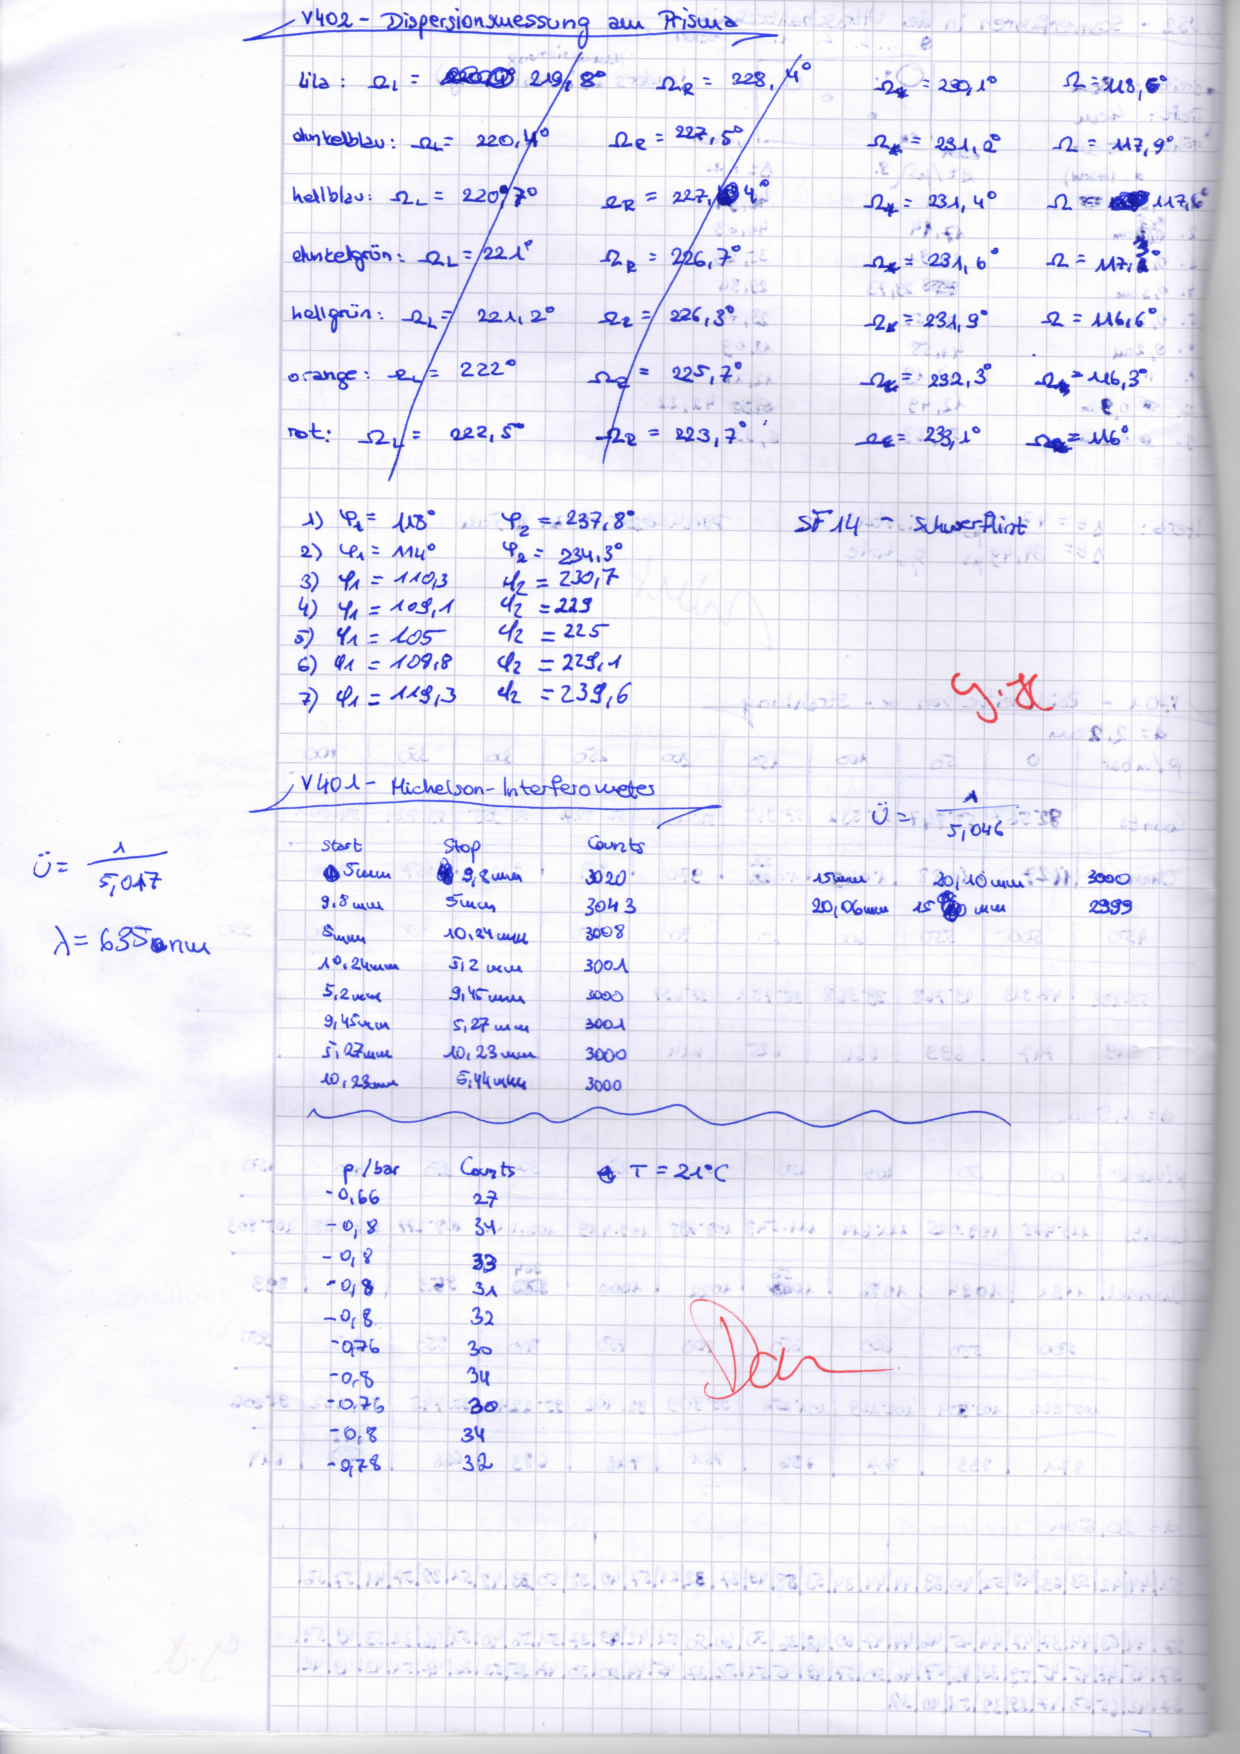
\includepdf[pages=-]{Text/Bilder/Messungen.pdf}

\end{document}
